\chapter{Continuous Integration und Continuous Delivery} \label{ch:cicd}

Das Ausführen sich wiederholender Aufgaben führt oft zu Langeweile, was zu Fehlern und Fehlern führt. Ein erfolgreiches Entwicklungsteam vermeidet es, sich wiederholende Aufgaben zu erledigen, um seine Zeit und Kreativität in wichtigere Aufgaben zu investieren. Die Automatisierung ist eine der Lösungen, mit denen dieses Ziel erreicht werden kann. Automatisierung im IT-Bereich zielt darauf ab, Dienste und Anwendungen mit möglichst wenig menschlichem Eingreifen zu produzieren und bereitzustellen. Durch die Implementierung von Automatisierung können die Zuverlässigkeit, Effizienz und Geschwindigkeit der Verarbeitung verschiedener Aufgaben im Vergleich zur Ausführung durch den Menschen erheblich verbessert werden. Nach der Verbreitung automatisierter Prozesse und Methoden hat es begonnen, Softwareentwicklungsmethoden wie \textit{Continuous Integration und Continuous Delivery/Deployment (CI/CD)} zu unterstützen.

\section{Continuous Integration}

Zu Beginn müssen einige von J. Humble und D. Farley \cite{JezHumble2010} genannte Begriffe geklärt werden, um dieses Kapitel zu verstehen:

\begin{itemize}
	\item Der \textbf{Build}  ist eine Reihe von Vorgängen, die zum Erzeugen, Testen und Bereitstellen von Software ausgeführt werden.
	
	\item \textbf{Kontinuierlich (eng. Continuous)} ist ein Prozess, der niemals aufhört, sobald er einmal begonnen hat. Mit anderen Worten, es handelt sich um einen Prozess, der kontinuierlich abläuft und einen neuen Build durchführt, wenn Änderungen im Versionskontroll-Repository entdeckt werden, z. B. auf GitHub \footnote{https://github.com/} oder GitLab \footnote{https://about.gitlab.com/}.
	
	\item \textbf{Integration} ist in der Sprache der Prozess der Eingliederung, der als Eingliederung in eine größere Einheit definiert ist. In der Welt der Informatik ist Integration die Aktion, die durchgeführt wird, um separate Quellcodes zu kombinieren, um festzustellen, wie sie als Ganzes funktionieren.
	
\end{itemize}
\ \\
\textit{Continuous Integration (Kontinuierliche Integration)(CI)} ist eine Reihe von Regeln und Praktiken in der Softwareentwicklung, an denen Entwicklungsteams beteiligt sind \cite{Meyer2014}. Jedes Teammitglied übernimmt die Verantwortung für die tägliche Integration und Zusammenführung des entwickelten Codes. Unter dem Begriff der Continuous Integration werden viele Perspektiven und Vorteile gesehen. Durch den Einsatz dieser Methode wurde festgestellt, dass sie dazu beiträgt, die Probleme bei der Integration erheblich zu reduzieren, was es einem Team ermöglicht, Software harmonisch und schneller zu entwickeln \cite{Fowler2006}. Der Grund dafür ist laut M. Shahin und M. Barbar, dass CI Softwareunternehmen aller Größenordnungen kürzere und häufigere Release-Zyklen ermöglicht, die Produktivität ihrer Teams erhöht und die Qualität ihrer Software verbessert. Die Automatisierung der Softwareerstellung und der Unit-/Integrationstests ist in dieser Praxis enthalten \cite{Shahin2017}. Ein erfolgreicher CI-Prozess bedeutet daher, dass neue Änderungen am Code erstellt, getestet und konsistent in ein gemeinsames Repository in einem Versionskontrollsystem wie GitHub oder GitLab zusammengeführt werden \cite{RedHat2018}. Kurz gefasst, kontinuierliche Integration legt großen Wert auf automatisierte Tests, um sicherzustellen, dass die Anwendung nicht abbricht, wenn neue Übertragungen in den main-Branch integriert werden \cite{Atlassian}.

\section{Continuous Delivery und Deployment}

\textit{Continuous Delivery (Kontinuierliche Bereitstellung)(CD)} ist eine Erweiterung der Continuous Integration, da alle Codeänderungen nach der Build- und Test-Phase in Produktionsumgebungen bereitgestellt werden. Das heißt, dass zusätzlich zum automatisierten Testen einen automatisierten Freigabeprozess (Release) gibt, die jederzeit per Mausklick bereitgestellt werden kann. Theoretisch hat der Entwickler die Entscheidung, wann einen neuen Release bereitgestellt werden kann bzw. täglich, wöchentlich, oder monatlich. Wenn der Entwickler jedoch wirklich von den Vorteilen der Continuous Delivery profitieren will, Atlassian empfiehlt, die Delivery für die Produktion so früh wie möglich vorzunehmen, um sicherzustellen, dass kleine Chargen freigegeben wird, die im Falle eines Problems leicht zu beheben sind \cite{Atlassian}. Die Continuous Delivery prüft den Code automatisch, erfordert aber einen menschlichen Eingriff, um die Delivery der Änderungen manuell auszulösen \cite{GitLab:CD}.

\textit{Continuous Deployment (Kontinuierliche Verteilung)(CD)} ist ein weiterer Schritt über Continuous Integration hinaus, der ähnlich wie Continuous Delivery ist. Der Unterschied besteht darin, dass die Anwendungen automatisch bereitstellen können, anstatt Anwendungen manuell bereitzustellen. Bei diesem Verfahren wird jede Änderung, die alle Phasen der Produktionspipeline durchläuft, automatisch für die Kunden freigegeben. Es gibt keine menschlichen Eingriffe, und nur ein fehlgeschlagener Test verhindert, dass eine neue Änderung in der Produktion bereitgestellt wird \cite{Atlassian}. Nach Bestehen der automatisierten Tests können Änderungen an einer Anwendung innerhalb von Minuten nach deren Erstellung in Betrieb genommen werden \cite{GitLab:CD}. Der größte Vorteil der Continous Deployment ist, dass die Kunden die Verbesserungen direkt sehen können, in der die Qualität jeden Tag steigt, anstatt jeden Monat oder jedes Jahr \cite{Atlassian}. Die Abbildung ~\ref{fig:zusammenhandCICD} hebt die Zusammenhang von CI/CD hervor.

\begin{figure}[!htbp]%[bth] 
	\centering
	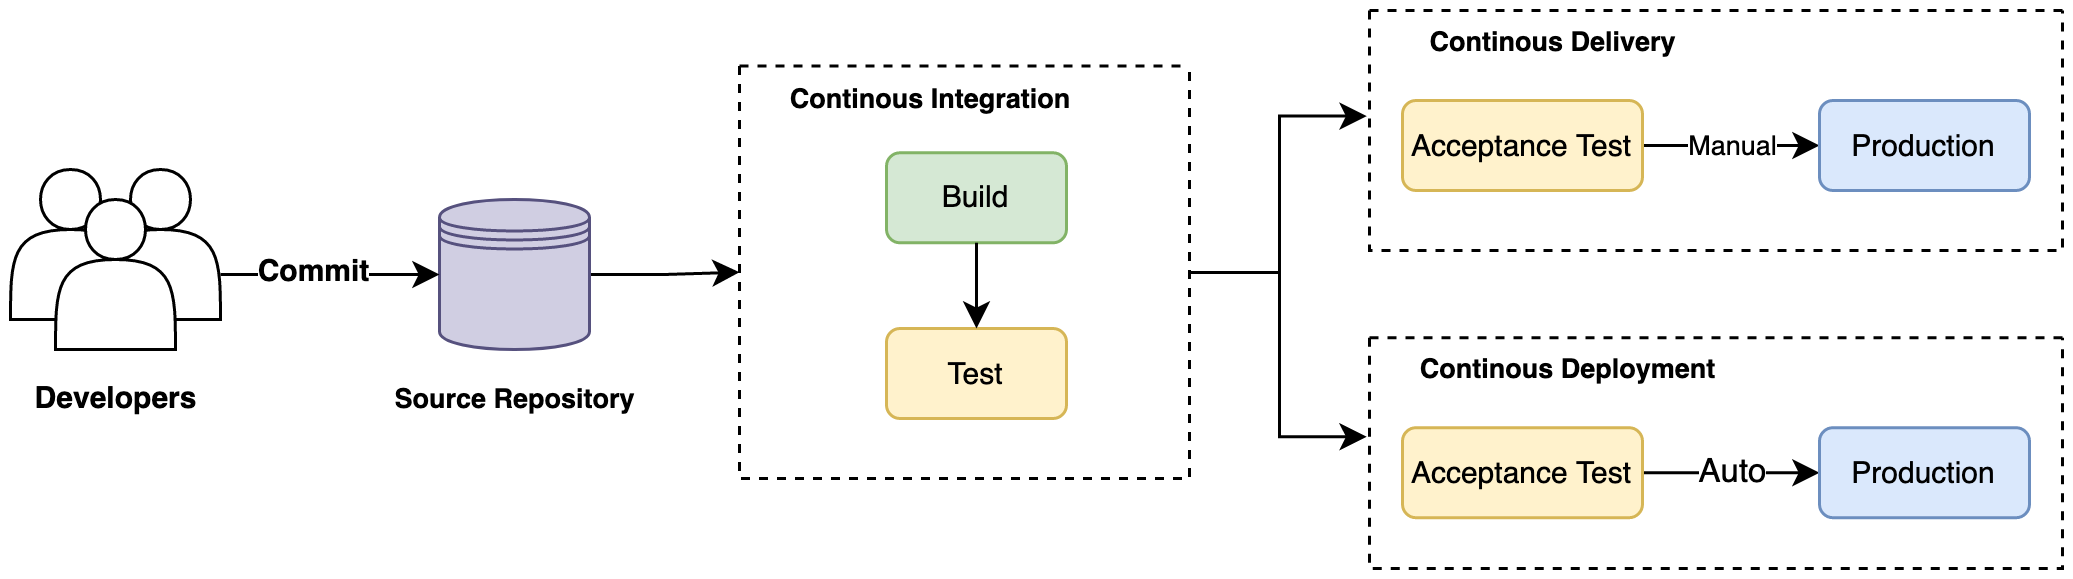
\includegraphics[width=0.9\textwidth]{Graphics/The-relationship-between-CI_CD.png}
	\caption{Die Zusammenhang zwischen CI/CD \cite{Shahin2017}}
	\label{fig:zusammenhandCICD}
\end{figure}

\pagebreak

\section{CI/CD Tools}

CI/CD-Tools können einem Team helfen, seine Entwicklung, Bereitstellung und Tests zu automatisieren. Einige Tools kümmern sich speziell um die Integration (CI), andere um die Entwicklung und Bereitstellung (CD), wieder andere sind auf kontinuierliche Tests oder verwandte Funktionen spezialisiert.

\subsection{Concourse CI}

\textit{Concourse CI} ist ein Open-Source-Tool zur kontinuierlichen Integration, das für die Bewältigung sich wiederholender Aufgaben entwickelt wurde. Um diese Aufgaben zu erfüllen, muss eine Automatisierungspipeline mit hilfe einer YAML-formatierten Konfigurationsdatei erstellt werden. Mit Hilfe von Concourse CI können Aufgaben, Ressourcen und Jobs, die sich von Zeit zu Zeit wiederholen, automatisch definiert und ausgeführt werden \cite{ConcourseCI:homepage}.

\begin{itemize}
	
	\item \textbf{Pipelines:} Entwickler müssen Pipelines erstellen, um bestimmte Aufgaben zu automatisieren. Dazu werden die Ressourcen und Jobs deklariert, die zur Erfüllung dieser Aufgaben erforderlich sind. Nach der Konfiguration können diese Pipelines feststellen, ob eine neue Version der definierten Resource veröffentlicht wurde. Wenn dies der Fall ist, stellt Concourse automatisch neue Builds für diese neu eingegebenen Jobs in die Warteschlange \cite{ConcourseCI:pipelines}. Ein gutes Beispiel für die Erkennung neuer Ressourcen-Aktualisierungen ist, wenn ein Entwickler neue Änderungen an einem Git Branch vornimmt, der in einem GitHub-Repository definiert ist. Solche Operationen veranlassen die Pipeline, einen neuen Build des Jobs zu erstellen.
	
	\item \textbf{Ressource (engl. Resource):} Ressourcen in Concourse sind Objekte, die in die Pipeline gezogen oder aus ihr herausgeschoben werden müssen. Nachdem diese Ressourcen richtig konfiguriert sind, überprüft Concourse sie regelmäßig auf neue Versionen und löst einen neuen Build aus, wenn ein Update gefunden wird \cite{ConcourseCI:Resources}. Eine der wichtigsten definierten Concourse Ressourcen ist git, die die Commits in einem Git-repository verfolgt \cite{ConcourseCI:git}. Eine weitere wichtige Ressource time, die steuert, wann die Pipeline ausgelöst wird, indem Zeitintervalle wie jede Stunde oder jede Mitternacht definiert werden \cite{ConcourseCI:time}.
	
	\item \textbf{Ressourcentypen (engl. Resource Types):} Concourse wird standardmäßig mit git-, time- und s3-Ressourcen ausgeliefert, was in den meisten Fällen ausreichen sollte. Wenn jedoch spezielle Ressourcen erforderlich sind, bietet Concourse eine Möglichkeit, externe Ressourcen zu erstellen, die nicht vom Concourse-Team bereitgestellt werden, sondern als Ressourcentypen definiert werden. Diese Ressourcentypen werden genauso behandelt wie native Ressourcen \cite{ConcourseCI:resourcetypes}. Zum Beispiel, CloudFoundry Community erstellte eine externe Ressource namens \footnote{https://github.com/cloudfoundry-community/slack-notification-resource}„slack-notification-resource“ für Concourse. Diese Ressource sendet Slack-Benachrichtigungen, wenn der Build erfolgreich und/oder nicht erfolgreich ist.
	
	\item \textbf{Aufträge (engl. Jobs):} Sie definieren das Verhalten der Pipeline und wie alle definierten Ressourcen durch die Pipeline vorankommen \cite{ConcourseCI:jobs}.
	
	\item \textbf{Aufgaben (engl. Tasks):} Concourse definiert Tasks als „die kleinste konfigurierbare Einheit in der Concourse-Pipeline“ \cite{ConcourseCI:tasks}. Entwickler können sich Concourse-Aufgaben als Funktionen vorstellen, die Arbeit erledigen.
	
\end{itemize}
\ \\
Listing~\ref{ConcourseHelloWorld} verdeutlicht, wie eine einfache Pipeline mit Concourse CI erstellt werden kann, die “Hello, world” ausgibt, wenn die Pipeline ausgelöst wird. Außerdem zeigt die Abbildung~\ref{fig:ConcourseHelloWorld}, wie das Ergebnis in Build Nr.01 aussieht. Nach erfolgreicher Ausführung des Jobs wird die Pipeline grün, ansonsten Rot.

\lstinputlisting
[caption={Concourse-Pipeline drückt 'Hello, world!' aus}, label=ConcourseHelloWorld]
{Listings/concourse-pipeline.yml}

\begin{figure}[!htbp]%[bth] 
	\centering
	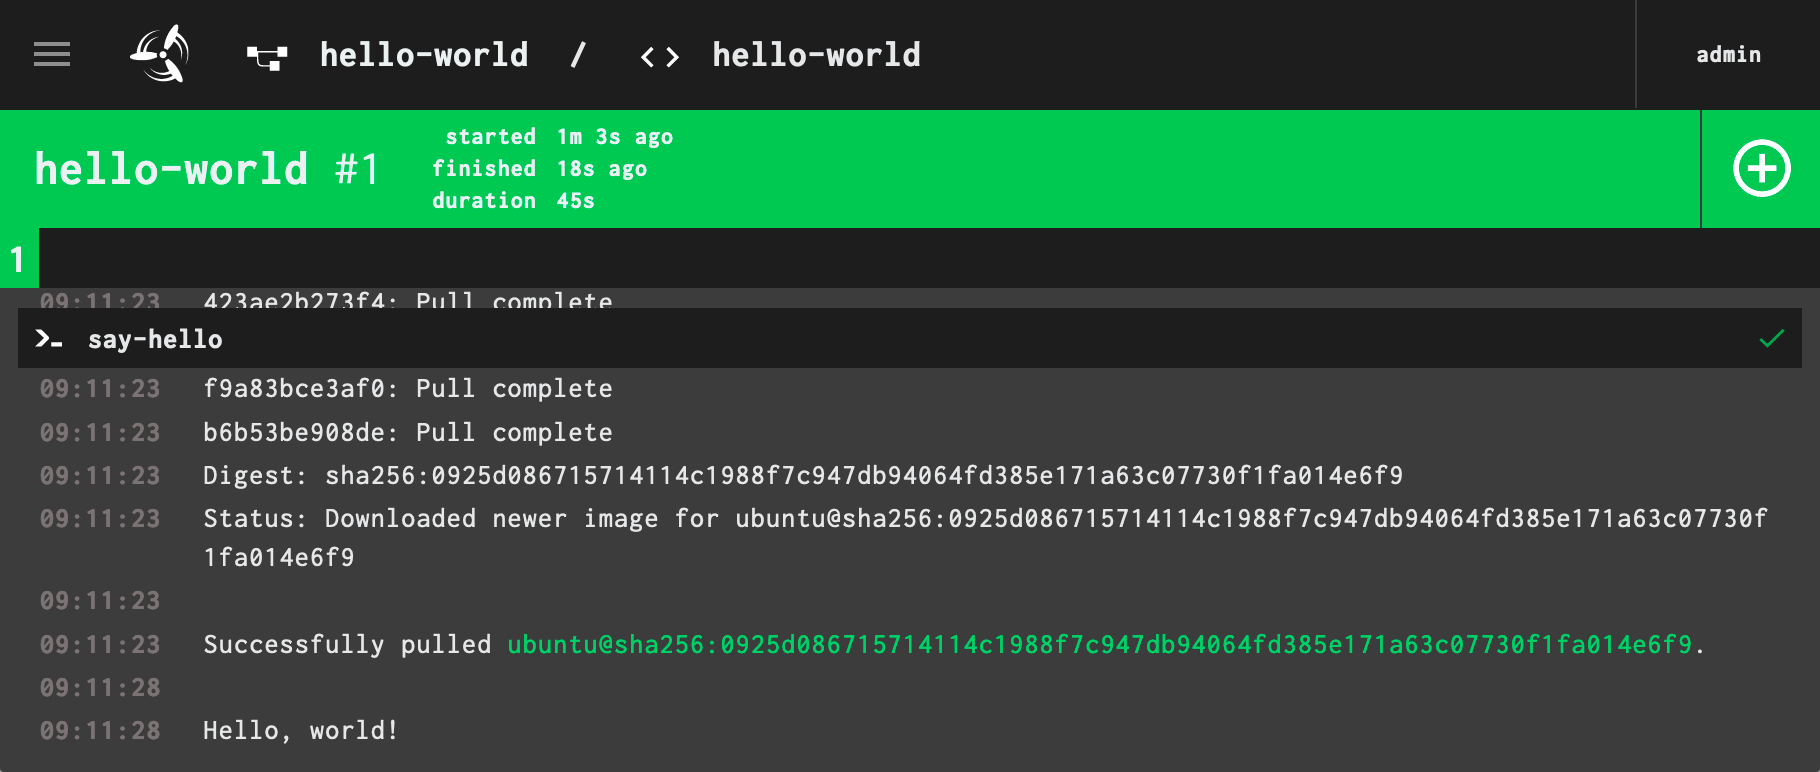
\includegraphics[width=0.9\textwidth]{Graphics/concourse-ci-job-success.png}
	\caption{Drucken von 'Hello, World!' nach Auslösen des “hello-world” Auftrag}
	\label{fig:ConcourseHelloWorld}
\end{figure}

\subsection{GitLab}\label{sub:gitlab}

\textit{GitLab} ist ein webbasiertes Git-Repository, das kostenlose offene und private Repositories bereitstellt. 
Außerdem ist GitLab eine vollständige DevOps-Plattform, die Entwicklungs-, Betriebs- und Sicherheitsteams in einer einzigen Anwendung vereint. Der Hauptvorteil der Verwendung von GitLab besteht darin, dass alle Teammitglieder in jeder Projektphase zusammenarbeiten können. Es bietet Nachverfolgung von der Planung bis zur Erstellung, um Entwicklern zu helfen, den gesamten DevOps-Lebenszyklus zu automatisieren und die bestmöglichen Ergebnisse zu erzielen. Immer mehr Entwickler verwenden GitLab aufgrund seiner umfangreichen Funktionen und der Verfügbarkeit von Code-Bausteinen. Aus diesem Grund wurde GitLab von verschiedenen großen Unternehmen wie Nvidia, Siemens und Cloud Native Computing Foundation benutzt \cite{GitLab:about}. 

Die gesamte Konfiguration der Pipeline wird in der YAML-Konfigurationsdatei \textit{.gitlab-ci.yml} gespeichert und besteht aus folgenden Hauptelementen:

\begin{itemize}
	
	\item \textbf{Aufträge (engl. Jobs):} Ein Auftrag in GitLab wird oft als "Build-Schritt" bezeichnet, da er der kleinste ausführbare Einheit in GitLab ist. Er kann eine Build- oder Kompilierungs- Deployment-aufgabe sein. Darüber hinaus kann ein Auftrag Unit-Tests ausführen und die Code-Qualitätsprüfungen beinhalten. Ein einzelner Auftrag kann mehrere Befehle (Skripte) enthalten, die ausgeführt werden können \cite{GitLab:jobs}.
	
	\item \textbf{Phasen (engl. Stages):} Jeder Auftrag gehört zu einer einzigen Phase. Eine Phase kann null, einen oder mehrere auszuführende Aufträge enthalten. Alle Aufträge in einer einzelnen Phase laufen parallel. Die nächste Phase wird nur dann ausgeführt, wenn alle Aufträge der vorherigen Phase erfolgreich abgeschlossen wurden oder als fehlgeschlagen markiert sind.
	GitLab hat drei standardmäßigen Phasen nähmlich \textit{build, testing} and \textit{deploy}. Wenn die Aufträge der Build-Phase erfolgreich abgeschlossen sind, geht GitLab zur Test-Phase über und startet alle Aufträge aus dieser Phase parallel. Wenn die Testphase abgeschlossen ist bzw. wenn alle Aufträge in der Testphase ausgeführt wurden, wird die Bereitstellungsphase ausgeführt. Phasen können manuell hinzugefügt oder neu definiert werden, in dem man das Stages-Array mit neuen Elementen in .gitlab-ci.yml definiert \cite{GitLab:stages}.
	
	\item \textbf{Pipelines:} Pipelines orchestrieren Jobs und Stages und fügen sie alle zusammen. Eine Pipeline wird ausgeführt, wenn eine neue Commit oder ein neues Tag gepusht wird, und führt alle Jobs in ihren Phasen in der richtigen Reihenfolge aus.
	
\end{itemize}
\ \\
Listing~\ref{GitLabHelloWorld} zeigt eine einfache gitlab-ci.yml-Datei, die eine Pipeline zum Drucken von „Hello, World!“ erstellt.

\lstinputlisting
[caption={Einfache .gitlab-ci.yml Datei zum Drucken von “Hello, World!”}, label=GitLabHelloWorld]
{Listings/gitlab-pipeline.yml}
\ \\
Nach einem erfolgreichen Lauf der Pipeline wird sie als bestanden (engl. passed) markiert, wie auf der Abbildung~\ref{fig:GitLabPipeLinePassed} steht.

\begin{figure}[!htbp]%[bth] 
	\centering
	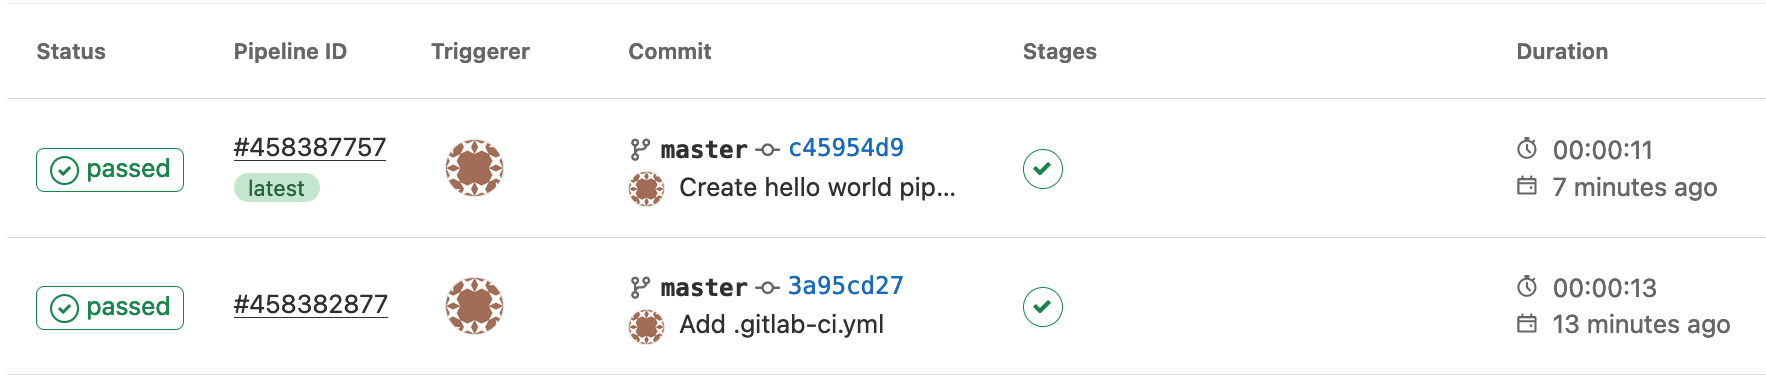
\includegraphics[width=0.9\textwidth]{Graphics/GitLab-passed_pipeline.png}
	\caption{Liste von Pipelines, die al bestanden (engl. passed) markiert wurde}
	\label{fig:GitLabPipeLinePassed}
\end{figure}
 
\pagebreak
Außerdem, wird diese einfache Pipeline wie auf der Abbildung~\ref{fig:GitLabHelloWorldPipeline} aussehen.

\begin{figure}[!htbp]%[bth] 
	\centering
	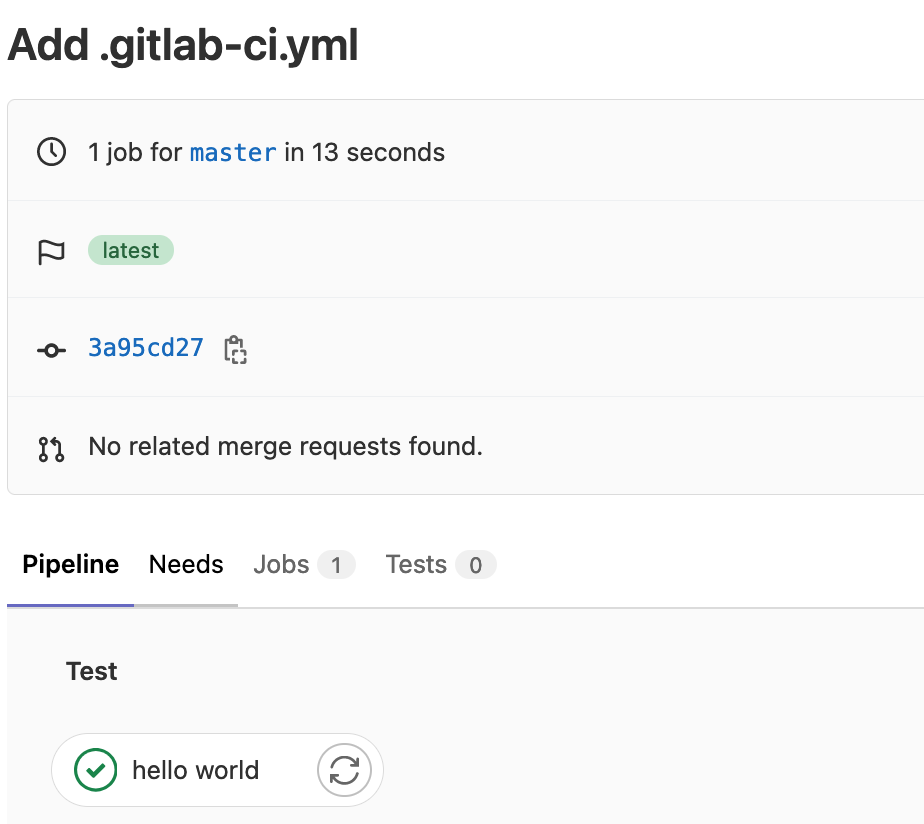
\includegraphics[width=0.7\textwidth]{Graphics/GitLab-helloWorld_pipeline.png}
	\caption{Einfache hello world pipeline in GitLab}
	\label{fig:GitLabHelloWorldPipeline}
\end{figure}
\ \\
Für weitere Informationen hat der Entwickler die Möglichkeit, einen Blick auf den Pipeline-Build zu werfen, der der Abbildung~\ref{fig:GitLabPipelineBuild} ähnlich sieht.

\pagebreak
\begin{figure}[!htbp]%[bth] 
	\centering
	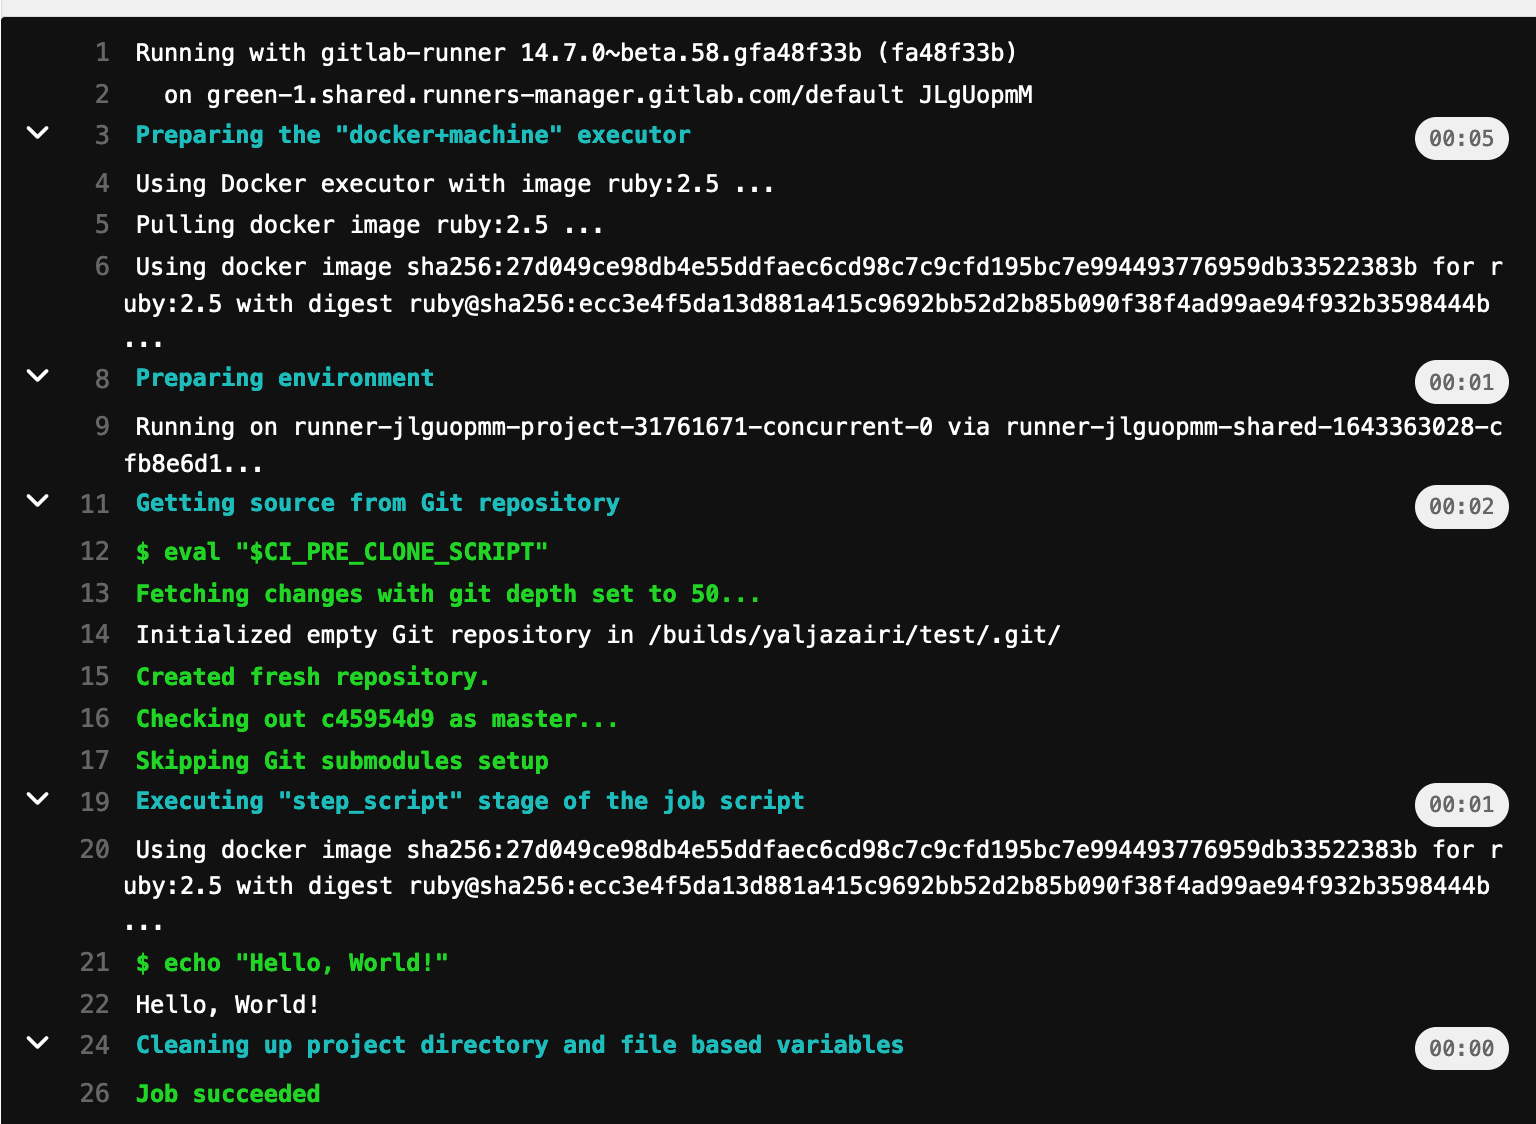
\includegraphics[width=0.9\textwidth]{Graphics/GitLab-pipeline-job-build.png}
	\caption{GitLab Pipeline-Build vom hello world Job}
	\label{fig:GitLabPipelineBuild}
\end{figure}

\subsection{CircleCI}

\textit{CircleCI} ist eine Plattform für kontinuierliche Integration und Bereitstellung, die Entwicklungsteams bei der schnellen Veröffentlichung von Code und der Automatisierung von Build, Test und Bereitstellung unterstützt. CircleCI kann so konfiguriert werden, dass sehr komplexe Pipelines mit Caching, Docker Layer Caching, Ressourcenklassen und vielem mehr effizient ausgeführt werden \cite{CircleCI:homepage}.
CircleCI sendet auch eine E-Mail- oder Slack-Benachrichtigung über Erfolg oder Misserfolg nach Abschluss der Tests \cite{CircleCI:notifications}.Führende Unternehmen wie Docker, Heroku, Kickstarter, Nextdoor, Udemy, Coinbase und Cucumber haben ihren Entwicklungsprozess erfolgreich über CircleCI durchgeführt \cite{CircleCI:customers}. Auf diese Weise gelang es ihnen, die Lieferung zu beschleunigen und die Produktqualität zu verbessern. Außerdem ist die Konfigurationsdatei vom CircleCI in YAML geschrieben und das Tool unterstützt viele Programmiersprachen. CircleCI bietet 1.000 Build-Minuten pro Monat und unbegrenzte Repos in einem kostenlosen Plan. Allerdings, stehen Skalierbare bezahlte Pläne zur Verfügung, wenn die kostenlose Plan nicht reicht \cite{CircleCI:pricing}.

\subsection{Jenkins}

\textit{Jenkins} ist eines der führenden Open-Source-Tools für \ac{CI/CD}. Es ist in Java geschrieben und verfügt über 300 Plugins zur Unterstützung der Erstellung und Prüfung jedes Projekts. Außerdem, unterstützt Jenkins alle wichtigen Sprachen und können seine Pipelines über \textit{Jenkinsfile} konfiguriert werden. Allerdings, müssen die Entwickler, die Jenkins benutzen möchten, die Groovy \footnote{https://groovy-lang.org/} Programmiersprache beherrschen \cite{Jenkins:pipeline}.
